\documentclass[%
 aip,
 jmp,%
 amsmath,amssymb,
%preprint,%
 reprint,%
%author-year,%
%author-numerical,%
]{revtex4-1}

\usepackage{graphicx}% Include figure files
\usepackage{dcolumn}% Align table columns on decimal point
\usepackage{bm}% bold math
%\usepackage[mathlines]{lineno}% Enable numbering of text and display math
%\linenumbers\relax % Commence numbering lines
\usepackage{mathtools}
\usepackage{amssymb}

\DeclarePairedDelimiter\abs{\lvert}{\rvert}
\DeclarePairedDelimiter\norm{\lVert}{\rVert}
\begin{document}

\title[Laboratory of Computational Physics module b]{Data Visualization with t-SNE algorithm}% Force line breaks with \\

\author{Dainese Nicola, Mancone Stefano, Vidaich Francesco}
\begin{abstract}
In this assignment the aim is to test the usage and efficacy of the
t-stochastic neighbour embedding (t-SNE) algorithm for the purpose of
data visualization.
\end{abstract}
\maketitle

%TITOLO1: Visualization task and loss of information
\section{Visualization task and information}
Ideally, in a analysis project, one do not have to look at the data to
formulate an hypothesis. It is however impossible to create a model
without any insight about data. If previous knowledge is available, the
safest way is to use it to create a model and then test it with some kind
of metric. In absence of previous useful information, it is necessary
to look at the data in some way as a starting point for further analysis.
Here comes in visualization. The essence of the problem of visualizing a
dataset with $n$ features (where $n > 3$) is that we can't do it without
loss of information. This is because the samples that we want to represent
live in an $n$-dimensional space and we can dispose only of 2 or at most
3 dimensions to represent them.
The case with $n \leq 3$ is easy because we can visualize it in our
own space. With $n > 3$ we are forced to find a suitable combination of
the initial coordinates (features) which reflects in some way the structure
of our samples in feature space. Actually there is a case in which we can
do it almost without loss of information, and this is when some of the
features can only assume few values, like 0-1 in the simplest case.
In fact we can encode this features in the color of the points, or using
different symbols and sizes for the markers.
However in this way we can account only for one or two extra dimensions
and the price to pay is that the amount of information delivered in a
single graph is overwhelming.
Anyhow in this review we will focus only on the representation of samples
with all the features that are continuous.
The easiest approach to reduce the dimension of the samples minimizing
the loss of information is Principal
Component Analysis (\textit{PCA}), where directions of most variance in the
covariance matrix of the dataset are found. This can be used to find
the most significant directions along which samples are distributed.
Significance is understood in the sense that direction with small variance
can be assumed as noise and therefore eliminated.
The most limit aspect of \textit{PCA} is that the transformation of the data
is linear and thus it cannot be used with datasets with a complex structure
like, for example, spirals.

%TITOLO2:  t-stochastic neighbour embedding (t-SNE)
\section{t-stochastic neighbour embedding}
In this report we practice with a more sophisticated method for data
visualization, that is called t-stochastic neighbour embedding (t-SNE).

The idea of stochastic neighbor embedding is to associate a probability
distribution to the neighborhood of each data point in the feature space ($x \in
 \mathbb{R}^n$) using a gaussian likelihood
 \[
p_{i|j} = \frac{\exp{(-\norm{x_i - x_j}^2/2\sigma^2_i)}}{\sum_{k \ne i} \exp{(-\norm{x_i - x_j}^2/2\sigma^2_i)}}
 \]
This implies that only points that are nearby $x_i$ contribute to its
distribution. To account this effect a symmetrized distribution $p_{ij} =
(p_{i|j} + p_{j|i})/(2N)$ is used. This guarantees that $\sum_{j}p_{ij} >
1/(2N)$ for all data points making each data point significant contribute
to the cost function to be defined below.
t-SNE algorithm constructs a similar probability distribution $q_{ij}$ in
a low dimensional latent space ( $y \in \mathbb{R}^{n'}$ where $n' < n$
is the dimension of the latent space)
\[
q_{ij} = \frac{(1+\norm{y_i - y_j}^2)^{-1}}{\sum_{k \ne i}(1+\norm{y_i - y_j}^2)^{-1}}
\]
Here $q_{ij}$ is chosen to be a long tailed distribution. This preserves
short distance information while strongly repelling two points that are
far apart in the original space. The last step is to find the latent
space coordinates $y_i$. In order to achieve this t-SNE algorithm minimizes
the Kullback-Leiber (KL) divergence between $q_{ij}$ and $p_{ij}$
\[
C(Y) = D_{KL}(p||q) = \sum_{ij}p_{ij} \log{(\frac{p_{ij}}{q_{ij}})}
\]

via gradient descent.
In order to acquire insight about how the t-SNE algorithm works we did
some experiments with the \textit{sklearn.manifold.TSNE}
class from scikit learn library.
Here the important hyperparameters that we can tune are:

\begin{itemize}
\item \textit{n\_components} defines the dimension of the latent space;
\item \textit{perplexity} sets the local entropy, which determines the
$\sigma_{i}$ in the gaussian likelihood;
\item \textit{early\_exaggeration} controls how much distance in the embedded
space will be between natural clusters in the original space;
\item \textit{learning\_rate} fixes the learning rate in the gradient descent;
\item \textit{n\_iter} is just the number of gradient updates;
\item \textit{n\_iter\_without\_progress} and \textit{min\_grad\_norm} are
just early stopping parameters;
\item \textit{init} can be chosen between "random" and "PCA".
\end{itemize}

In order to experiment with this algorithm we were provided five different
datasets of samples generated from five unknown functions.
In every dataset there are five features and a color, which varies with
continuity on the manifold from which the samples were generated.
We start considering the first dataset, in order to understand how the
different hyperparameters of the algorithm work.
We have initially plotted the different pairwise scatter plots of the
five features to get an idea about the structure of the dataset.
Verified the non-trivial disposition of the samples, we applied the t-SNE
transform for different choices of the hyperparameters.
Since from the documentation seems that the perplexity is the main
discriminator about how the algorithm behaves, the runs have been
performed choosing the perplexity between $[2, 5, 50, 100]$ and changing
the others hyperparameters one at the time.

\begin{figure}[h]
 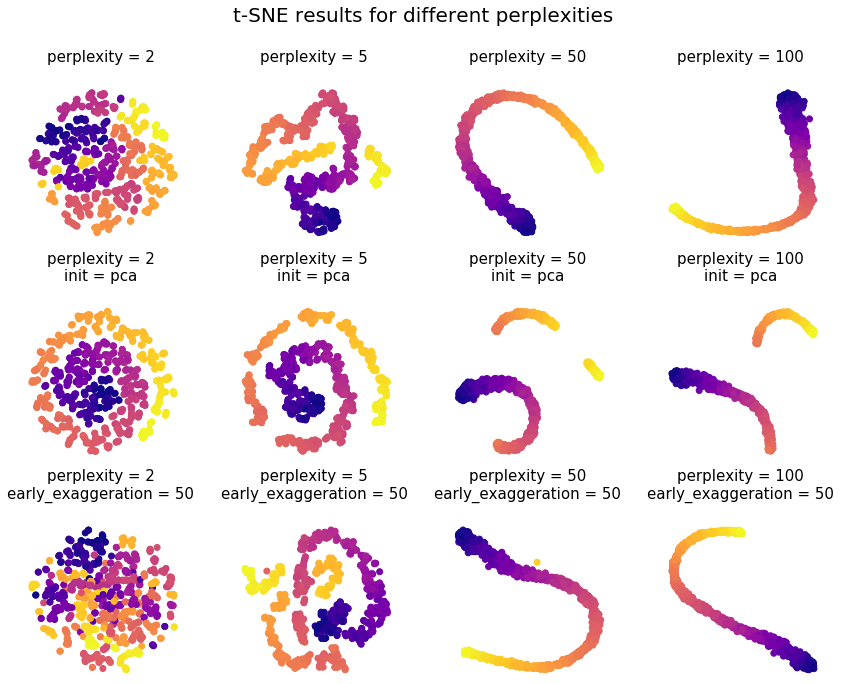
\includegraphics[scale=0.26]{images/t-SNE.png}
 \caption{t-SNE algorithm with perplexity in [2,5,50,100], init as PCA and early exaggeration 36}
 \label{fig:tsne}
\end{figure}

In Figure~\ref{fig:tsne} we have reported the runs with only changes in
perplexity, with \textit{init} chosen as PCA and with the early exaggeration
parameter set to $36$. It is clear that a different choice of perplexity
parameter lead to a qualitative different result. The strategy that
we find most efficient is to use all the different results together for
infer some properties of the data. For example in this case, from the
the runs with all default values and perplexity $[5, 50, 100]$ seems
clear that the structure of the data develops on a single dimensional
manifold. Looking instead at the runs with initialization with PCA, we
can see that it appears a structure similar to a spiral. Taking together
these two piece of information we already have a pretty good idea about
the structure of the first dataset.

From other experiments, whose graphs we do not report, we observe that,
unlike what happens with other algorithms, in this case most of the
hyperparameters choices lead only to slightly different results.
For example the \textit{learning\_rate} best choice is the default one
and the behaviour does not change, unless it is varied of order of magnitude,
in which case one will get very poor results.

%TITOLO3: t-SNE and unsupervised color-labelling
\section{t-SNE and unsupervised color-labelling}
A spontaneous objection to this strategy is that we used the colors we were given to
understand the structure of the data, but they are a labeling feature we
do not have in real world visualization tasks. It is then interesting
to find a strategy for coloring the samples, which otherwise would look colorless
and more difficult to interpret.
Since the embedding can be performed to an arbitrary latent space, one can
choose a one dimensional latent space, map the output coordinate in the
interval [0,1] and use it  as color labels also for 2D and 3D target spaces;
we will refer to this method as forced projection.
This seems more promising that simply using the last coordinate from
an $n'$-dimensional space as color, because if $n'=1$ the algorithm is forced to infer a meaningful
structure for the color. This however has a really limited utility; in
fact it loses effectiveness as soon as the dataset topology leaves the
case of a simple non-closed curve. Another strategy is to
perform a k-means clustering choosing a priori or iteratively the number of
interesting components and then using the mapped colors to look at the data
in different realizations of the t-SNE algorithms.
%A more refined approach can be done using a hierarchical clustering technique:
%the idea is to start considering each point as a cluster and then with a certain criteria
%merging neighbor clusters iteratively until a fixed number of clusters k (specified as input)
%is reached. For example single linkage clustering  will be very  effective, because minimizes
%the distance between the closest observations of pairs of clusters,

%performed in a space in which components
%that are disconnected in the original space remain disconnected in the latent space

\begin{figure}[h]
 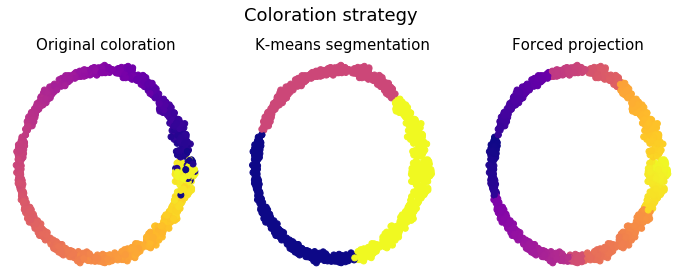
\includegraphics[scale=0.26]{images/coloration.png}
 \caption{Different coloration strategies for unsupervised learning}
 \label{fig:coloring}
\end{figure}

In Figure~\ref{fig:coloring} we had taken the second dataset we had
available to test the efficacy of the two methods. As it can be
seen, while the k-means method is quite coarse, the forced projection method
is not much reliable. Therefore, even if the k-means method is not
perfect, can be effective to gain insight in those cases where a previously
given coloration was not provided.

\begin{figure}[h]
 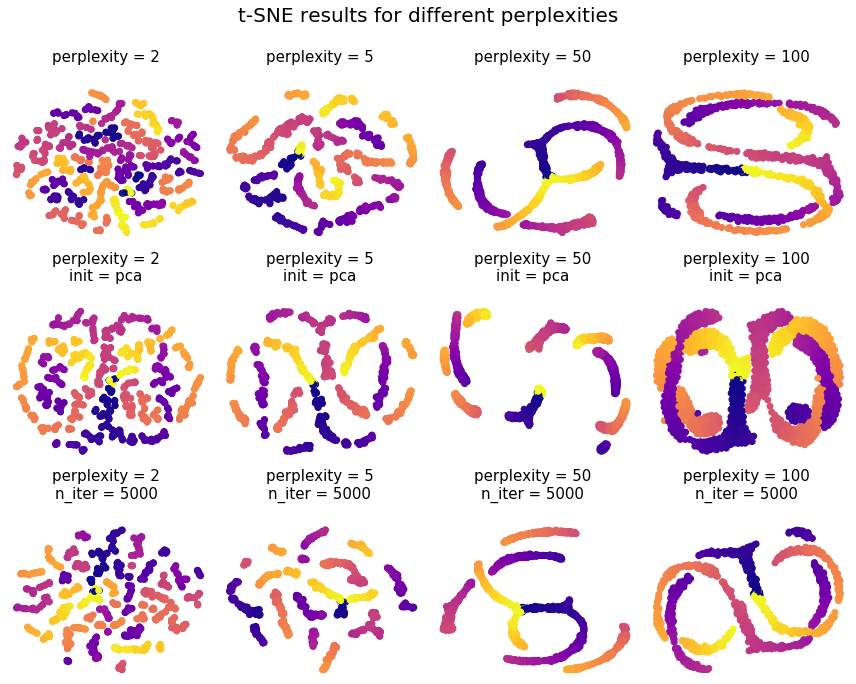
\includegraphics[scale=0.26]{images/fifth.png}
 \caption{Fifth dataset rappresentation in different 2D latent spaces}
 \label{fig:fifth}
\end{figure}

The last dataset on which we did some tests was the fifth. In Figure~\ref{fig:fifth}
we show the results of executing the algorithm with some hyperparameters.
The data structure however remained not easly understandable. After some
other attemps we decided to set the latent space dimension to 3. The
obtained result are shown in Figure~\ref{fig:3d}.
Is then immediately clear what the structure of the fifth dataset is.
Also the 2D plots in Figure~\ref{fig:fifth} are now more interpretable.
\begin{figure}[h]
 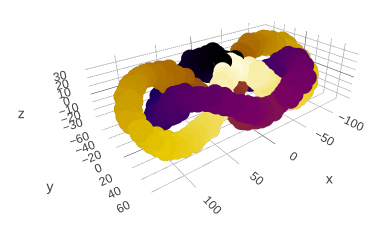
\includegraphics[scale=2]{images/3d.png}
 \caption{Fifth dataset rappresentation in a 3D latent space}
 \label{fig:3d}
\end{figure}




%TITOLO4: t-SNE scope and limitations
\section{t-SNE scope and limitations}
% da qui in poi è concettualmente confuso il tutto
The last example highlights one t-SNE algorithm limits. If the samples have
an intricate structure, for example presents some knots, the embedded space
dimension must be large enough to represent these complexities topologically.
But, although this is actually a limitation, we are already far ahead of
other unsupervised algorithms such as k-means clustering in terms of
applicability. If however one wants to find an algorithm that is not
affected by this limit, one should take a look to the k-Nearest-Neighbors
or  hierarchical clustering which could be used together with t-SNE.

The last tests we performed were with the Modified National Institute of
Standards and Technology (MNIST) dataset of handwritten digits. This
is a standard classification dataset and thus it is used as a benchmark
for classification problems. Our goal is to understand if with these %<-HERE
unsupervised techniques we can recognize a structure that can then be
learned in principle with supervised learning.

Every sample of this dataset is a $28 \times 28 = 784$
pixels image where every pixel is a number between $0$ and $255$ which
correspond to the pixel gray scale. We used the t-SNE algorithm on
$6000$ samples over $10000$ iterations with a perplexity of $30$ and a
learning rate of $200$. Then we used the so obtained coordinates
to train a k-means algorithm; finally we labelled each cluster with the
corresponding digit, to check if we got to catch the structure of the
dataset. %<-HERE

%using the labels of the training samples (however this is
%not necessary nor possible in an unsupervised learning task, but the MINST dataset
%of course is used for classification tasks

\begin{figure}[h]
 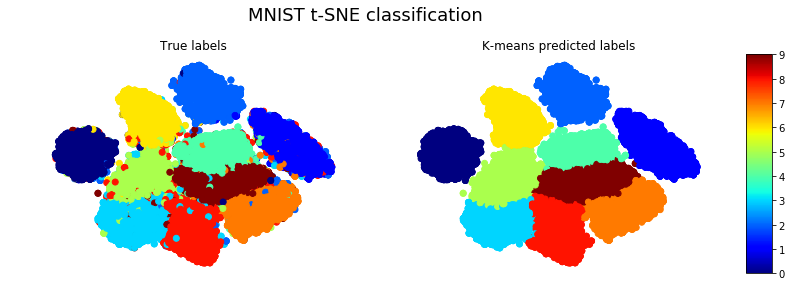
\includegraphics[scale=0.3]{images/MNIST.png}
 \caption{MNIST dataset classification with t-SNE e k-means algorithms}
 \label{fig:MNIST}
\end{figure}

With this very naive method we got an accuracy of $95.3\%$. Which mean
that the actual structure has been obtained quite accurately.
One thing to note here is that, because the digit clusters are not very
separated perform the k-means algorithm with exactly $10$ centroids lead
to poor results because the algorithm collocate them in unfavorable
positions. As it is shown in Figure~\ref{fig:centroids}
a solution can be initialize the algorithm with a doubled number of
centroids and then reduce the effective number of clusters using a
democratical approach to assign to each cluster the corresponding label.

\begin{figure}[h]
 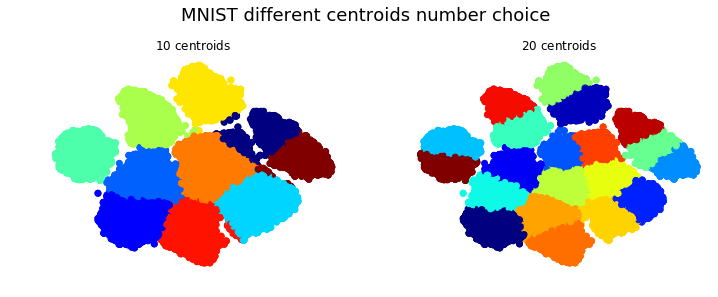
\includegraphics[scale=0.3]{images/centroids.png}
 \caption{Different cluster representation conditioned by the centroids number choice}
 \label{fig:centroids}
\end{figure}

% TITOLO5: Conclusions
\section{Conclusions}
We had therefore sperimented with the usage of the t-SNE algorithm.
We had seen that despite having some limitation (no free lunch theorem)
it is very useful to gain insight about the structure and the disposition
of the data. %As in other contexts however, the most effective method is to
%combining multiple methods together and use intelligence.
Its usage is particularly recommended when data belong to a low dimensional
manifold without complex topological behaviour, which is usually the case.
At the end of the day its scope is limited only to visualization tasks, that are the ones for which it is designed.
Instead t-SNE can not be used in learning tasks because it does not create a map between the feature space and the embedded
space as, for example, the PCA. It only act directly on the sample points
so there is not a obvious way to use it for dimensionality reduction.
Beyond then to its use for data visualization it has limited use also
due to his heavy computational cost.

% ti metto qui quello che ti ho scritto su whatsapp, poi discuteremo con calma su cosa tenere della parte sopra e su come integrare le due.
%TITOLO: t-SNE and Learning Tasks
%We have seen that the expressive power of t-SNE is huge for what concerns data visualization, in particular if combined with some labels according to which one can color the data. In this section we want to highlight some methods to



%Allora io inizialmente avevo proposto di usare tecniche di unsupervised learning per colorare automaticamente i risultati del t-SNE e l'idea è che qualsiasi sia il risultato del t-SNE riesci ad ottenere un labelling automatico che poi visualizzi come colore.
%Il fatto è che la visualizzazione è un fine e non uno strumento, quindi è sempre una cosa a colpo singolo e non ti importa di "imparare" la trasformazione che ti permette di visualizzare i dati.
%La stocasticità dell'algoritmo lo rende pesante computazionalmente e non apprendibile, quindi è automaticamente escluso da tutti i task di apprendimento.
%Quindi tutto il discorso fatto sulla colorazione ci sta, quello sul MNIST secondo me hai ciccato concettualmente l'applicazione. Cioè è vero che hai classificato bene i dati di training, ma ha la stessa utilità dell'assegnare ad ogni dato di training il suo label, perché entrambi i metodi non hanno potere predittivo e quindi non hanno senso
%Quindi nuovamente quello che puoi fare di sensato con il dataset del MNIST è utilizzare la trasformazione t-SNE e poi qualsiasi tecnica di clustering per visualizzare la difficoltà intrinseca del fare previsioni su quel dataset
%Inoltre ogni tentativo di riportare indietro quello che hai imparato nello spazio ridotto è destinato a fallire, perché la metrica globale dei due spazi non è conservata. Ti faccio un esempio: io posso segnarmi per ogni cluster quali punti vi appartengono e calcolarmi il cluster nello spazio originale come la media delle coordinate originali dei punti che vi appartengono (l'identità dei punti è conservata e quindi quell'informazione riesci a riportarla indietro). Ma se tu hai un nastro ripiegato su di sè in vari strati idealmente con il t-SNE tu lo tiri alle estremità per "stenderlo" e poi raggruppi i punti, ma tornando indietro strati diversi sono più vicini (per la metrica euclidea) tra loro che punti sullo stesso strato e quindi non riesci a fare previsioni basate sui cluster.
%Potresti fare scelta di maggioranza, tipo guardando i 10 punti del training più vicini (sempre secondo la distanza euclidea) e assegnando come predizione il label della maggioranza, ma per fare una previsione dovresti sempre avere i dati del training sotto mano e scorrerli tutti per calcolare le distanze, quindi una previsione diventa di ordine O(n) almeno, invece che O(1) nel caso di qualsiasi previsione sensata in cui impari i parametri e poi li tieni fissati.


\end{document}
%
% ****** End of file aipsamp.tex ******mango culo
